\section{Naive Bayes Nearest Neighbor} % (fold)
\label{cha:naive_bayes_nearest_neighbor}

\todo[inline]{short introduction of a paragraph or so? SEEMS TO BE OK, PERHAPS CUT SOME OF THE WORK ON BEHMO A LITTLE, MAKE A SUBSEC ON ..?(forgot what)}

\subsection{$k$-Nearest Neighbor Classification} % (fold)
\label{sub:_k_nearest_neighbor}

The $k$-Nearest-Neighbor algorithm is one of the earliest approaches for classification in machine learning. Given a set of items $n \in \mathcal{N}$, labeled with a designated number of classes $c_n \in \mathcal{C}$, an unlabeled query item $q$ and a distance measure to calculate pairwise differences between items $d(x_1\|x_2)$, the nearest neighbors of $q$ are the $k$ items in $\mathcal{N}$ for which $d(q\|n)$ is lowest. In turn, sets $\text{NN}_c(q)$ contain those nearest neighbors of $q$ that belong to class $c$. This way, $k$NN classification comes down to
\begin{align}
    \hat c_q &= \argmax_c |\text{NN}_c(q)|,
\end{align}
being the class of which the most items are within the $k$ nearest neighbors of $q$.

In contrast to other classification algorithms, $k$NN is relatively simple. It does not require any training to make a model from the labeled images. The algorithm only estimates the probability density of the classes locally, within $k$, which means it does not assume a global probability density distribution underneath the data, which makes it non-parametric, and a cheap\JanTodo{in what sense (or remove)?} way of making a non-linear classifier.

\subsection{Naive Bayes Classification} % (fold)
\label{sub:NB}

Naive Bayes is another rather simple classification algorithm, which is based on the idea that a simplification of Bayes' Theorem can be made using the assumption that all features of an item $d_{n,i} \in \mathcal{D}_n$ appear conditionally independent of each other. This means that $p(d_{n,i} | c_n, d_{n,j}) = p(d_{n,i}|c_n)$ is assumed for all $n,c,i,j, i\neq j$. 

If Bayes' Theorem is modeled to predict the probability of a class $c$ of an item $q$, we can say
\begin{align}
    \label{eq:bayes}
    p(c|q)      &= \frac{p(q|c)\,p(c)}{p(q)}\\
                &\propto p(q|c)\,p(c),
\end{align}
because the probability is to be compared among all classes $\mathcal{C}$, for the same item $q$, which makes $p(q)$ constant. Furthermore, if $q$ is represented by $m$ features $d_q$, \eqref{eq:bayes} can be rewritten as
\begin{equation}
    p(c|d_{q,1},\dotsc,d_{q,m}) = p(d_{q,1}, \dotsc,d_{q,m}|c)\,p(c),
\end{equation}
which is equivalent to the joint probability
\begin{align}\begin{split}
    p(c|d_{q,1},\dotsc,d_{q,m}) &\propto p(c,d_{q,1}, \dotsc,d_{q,m})\\
        &\propto p(c)\,p(d_{q,1}|c)\, p(d_{q,2}|c,d_{q,1}), \dotsc,p(d_{q,m}|c,d_{q,1},d_{q,2},\dotsc,\\&\quad d_{q,m-1}).
    \end{split} 
\end{align}
By the conditional dependence assumption made above, this can be reduced into
\begin{equation}
    p(c|q) \propto p(c)\prod_{i=1}^m p(d_{q,i}|c).
\end{equation}
With this equation, a decision rule can be made as follows
\begin{equation} \label{eq:map}
    \hat c_q = \argmax_c \frac{1}{m}\,p(c)\prod_{i=1}^m p(d_{q,i}|c),
\end{equation}
which is called a maximum a-posteriori (MAP) classifier. In this formulation of a classification problem, a probability density estimation is needed to model all features. All kinds of distributions can be used for this.

\subsection{Boiman's NBNN} % (fold)
\label{sub:boiman_s_nbnn}
Boiman \emph{et al.} \cite{boiman2008defense} coined the term Naive Bayes Nearest Neighbor (NBNN) for their image classification algorithm, that used a combination of Nearest-Neighbor (NN) and Naive Bayes to classify images in a multi-class setting. The approach works well because of the non-parametric character of the approach, which means no parameter learning is required. This makes it easy to use the method on a problem with a large number of classes (parametric methods typically model multi-class problems as multiple 2-class problems), and that the risk of overfitting is small because there are no parameters\JanTodo{NRK?} to be overfit. The authors achieved results competitive to the state of the art Bag of Features (BoF) methods because of two requirements their method meets: (\emph{i}) Avoiding feature quantization and (\emph{ii}) the use of image-to-class distance instead of image-to-image distances. They theorize that earlier attempts to use NN \todo[fancyline]{references} for image classification failed because these do not meet both requirements.

\begin{figure}[hbt]
    \centering
    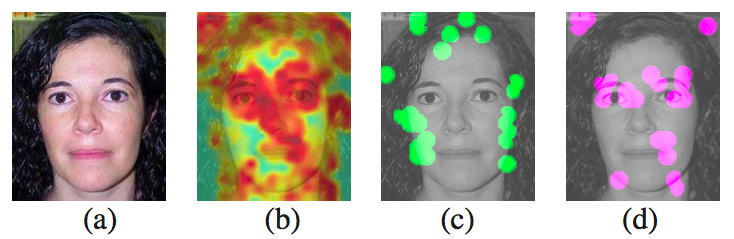
\includegraphics[width=0.8\textwidth]{QuantizationError}
    \caption{Quantization Error.}
    \label{fig:quantization_error}
\end{figure}

Feature quantization is a means of creating compact image descriptions, such as the ones used in the BoF methods. In BoF, all descriptors of an image are clustered into visual words, and histograms are constructed counting the occurrence of each word in an image. Image matching is based on comparing these histograms. This being useful in learning-based methods, quantization is harmful for a nearest neighbor approach because the most informative descriptors get the highest quantization error while being necessary for finding nearest neighbors. This becomes clear when the observation is made that for a descriptor to be more informative, it should appear only at certain circumstances, ideally only in images of one class. They should be fairly well recognizable among other descriptors, and therefore they tend to be outliers in descriptor space. When quantizing, these descriptors will mostly be incorporated into visual words that are rather unlike these descriptors, resulting in a large quantization error. In Figure \ref{fig:quantization_error}, the effects of this are illustrated. \todo{explain image, perhaps change image to own.}

In learning-based methods, like SVM, this disadvantage is outweighed by the benefit of dimensionality reduction which allows training on a large data set. Furthermore, when learning a BoF model, the problem itself is mitigated too. Therefore, NBNN uses every single descriptor of each image to perform NN on.

Kernel methods such as SVM are based on image-to-image distances to create decision boundaries. For each image in the training set, a histogram of visual words is built, based on the features that appear in the image, and are matched with the visual words that resulted from quantizing all training features. 
In a nearest neighbor approach, image-to-image distances do not enable much generalization, as no inference is done from the training images and their features. This would mean only test images close to known images will be classified correctly. Therefore, image-to-class distances should be used. While an image might be far removed from all others of a certain class, the individual features might all be close to features of different images of this class, making the image-to-image distances to a class large, but the image-to-class distance short. \cite{wang2009learning} Figure \ref{fig:im2im_vs_im2cl} shows the difference between image-to-image distance and image-to-class distance.\todo{Make a better embedding of the image in the text.}

\begin{figure}[hbt]
    \centering
    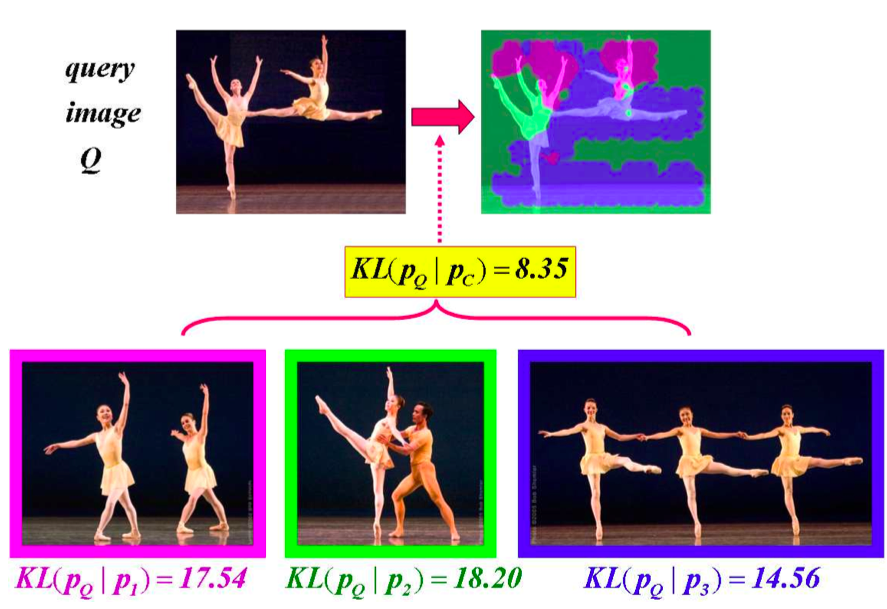
\includegraphics[width=0.8\textwidth]{Im2imVsIm2cl}
    \caption{Image to class distance vs image to image}
    \label{fig:im2im_vs_im2cl}
\end{figure}


Using the main points of no quantization an image-to-class distances, $k$-nearest neighbor can be performed for individual features, per class. Note that in this way, it is impossible to use $k$NN as a classifier, because no discrimination can be made between the classes. It is however useful to be able to compare the distances of a feature to the nearest neighbors in each class. this is used as the input of a Naive Bayes classifier.


The NBNN decision rule is defined under the Naive Bayes assumption of Section \ref{sub:NB}. The MAP classifier from \eqref{eq:map}, when assuming uniform priors $p(c)$ over all classes, simplifies to Maximum Likelihood (ML) classifier 
\begin{align}
    \hat c &= \argmax_c \frac{1}{m}\prod_{i=1}^{m} p(d_{q,i}|c)\\
           &\propto \argmax_c \frac{1}{n}\sum_{i=1}^{n} \log p(d_{q,i}|c),
\end{align}
Where the last formulation as a sum of log-probabilities is used in practice to compensate for the low probabilities typical for this classifier, which may cause rounding errors in computer applications.

Using the notion that NN classification tends to the Bayes optimal classifier when the sample size tends to infinity\cite{cover1967nearest, boiman2008defense}, dense sampling can be used to get a high number of descriptors per class from the training set $Z = |\mathcal{D}_c|$. The class conditional probability of a feature $p(d_q|c)$ can be modeled using Parzen likelihood estimation, where
\begin{equation} \label{eq:parzen}
    \hat p(d_q|c) = \frac{1}{Z}\sum_{j=1}^L K(d_q-d_{c,j}).
\end{equation}
Parzen kernel function $K(\cdot)$, typically Gaussian, defines the distance between query descriptor $d_{q}$ and labeled descriptor $d_{c}$. When $Z$ goes to infinity, $\hat p(f|c)$ approaches $p(f|c)$. 

This approach entails calculating the distance of $d$ to all $Z$ descriptors of each class, which would be very costly. Because only a small minority of the descriptors can be expected to be significantly close to $d_q$, taking into account only the nearest descriptors is a safe approximation, which enables using nearest neighbors (NN) to find these descriptors. Even more so, Boiman shows that taking only the 1 nearest neighbor hurts performance but little. Because of this the Parzen estimate of $d_q$ to class $c$ reduces to the distance of $d_q$ to its nearest neighbor in $c$: $\|d_q - \text{NN}_c(d_q)\|^2$, resulting in the following log likelihood and classifier: 
\begin{align}
    \label{eq:nbnnloglikelihood}
    \log P(q|c) &\propto -\sum_{i=1}^m \|d_{q,i} - \text{NN}_c(d_{q,i})\|^2 \\
    \label{eq:nbnnclass}
    \hat c      &= \argmin_c \sum_{i=1}^m \|d_{q,i} - \text{NN}_c(d_{q,i})\|^2
\end{align}

Now, classification comes down to calculating descriptors for all images in each class and for the query image, estimating the nearest neighbor of each query descriptor for each class, calculating the sum of distances for each class for the query image and selecting the lowest distance. This approach is both very simple and intuitive. It also enables use of different kinds and combinations of descriptors.

% subsection boiman_s_nbnn (end)


\subsection{Limitations and Extensions} % (fold)
\label{sub:limitations_and_extensions}

Even though the algorithm of \cite{boiman2008defense} is very simple and requires no training phase, it does have scalability issues because of its dependence of as many individual descriptors as possible. Because all densely computed descriptors for each image in the training set have to be stored, and the nearest neighbor for each descriptor of each query image on each class has to be found, the memory usage is much higher than for example BoF methods, which use a more compact representation of images. Calculating NN can be sped up by using sophisticated Approximations of the Nearest Neighbor algorithm, such as \todo[fancyline]{cite FLANN, ANN, some detail about FLANN???}. The memory issue remains however.

Other limitations have been shown by various authors.\cite{behmo2010towards, wang2011improved,mccann2012local,tuytelaars2011nbnn,timofte2012iterative} Some authors \cite{behmo2010towards,wang2011improved} stress that NBNN is highly sensitive to differences in descriptor density over classes. Behmo \emph{et al.} for example state that this is caused by dropping the factor $\frac{1}{Z}$ from the classification rule, which normalizes for the descriptor density in the train set for a given class; compare Equations \eqref{eq:parzen} and \eqref{eq:nbnnloglikelihood}. This term is dropped because an equal kernel estimation is assumed, which does not hold for large differences in descriptor density over classes.\cite{behmo2010towards} Therefore, they propose to learn the density estimation parameters per class, variance $\sigma_c$ and normalization factor $Z_c$, as a linear problem. Rephrasing the general Parzen-based likelihood \eqref{eq:parzen} gives
\begin{align}
    - \log\big(p(d_q|c)\big) &= -\log\Bigg(\frac{1}{ Z_c}\exp\left( -\frac{ \|d_q - \text{NN}_c(d_q)\|^2}{2(\sigma_c)^2}\right)\!\Bigg) \\
    &= \frac{ \|d_q - \text{NN}_c(d_q)\|^2}{2(\sigma_c)^2} + \log(Z_c),
\end{align}
and subsequently rephrasing and re-parametrizing the Naive Bayes rule \eqref{eq:nbnnclass} gives
\begin{align}
    \hat c_q &= \argmin_c \sum_{i=1}^{m_q} \left(\frac{ \|d_q - \text{NN}_c(d_q)\|^2}{2(\sigma_c)^2} + \log(Z_c)\right)\\
    &= \argmin_c \alpha_c \sum_{i=1}^{m_q} \|d_q - \text{NN}_c(d_q)\|^2 + m_q\beta_c,
\end{align}
using $\alpha_c = \frac{1}{2(\sigma_c)^2}$ and $\beta_c = \log(Z_c)$. This new formulation models an affine transformation on the distance measure used in NBNN. These two parameters can be seen as corrections for each class on the bias that arises when classes with the same priors are not equally sampled.

$\alpha_c$ and $\beta_c$ can be estimated in a training phase, where the outcome of the vanilla NBNN distances are used as input for a linear energy optimization problem:

\begin{align}\begin{split} \label{eq:energy}
    E(W) = \sum_{j=1}^{K} \max_{c:c\neq c_j} \Big(1\,&+\,\alpha_{c_j} \sum_d \|d - \text{NN}_{c_j}(d)\|^2 + m\beta_{c_j}\\
    &-\,\alpha_{c} \sum_d \|d - \text{NN}_{c}(d)\|^2 + m\beta_{c}\Big)_{+},
\end{split}\end{align}

where $E(W)$ is the energy of the current parameter set $W$, containing all $\alpha$ and $\beta$, and the equation represents the difference between the distance of all images in $K$ to its true class $c_j$ and to the nearest other class $max_{c:c\neq c_j}$. If this distance is minimized for all images, the hinge loss of the NBNN classifier is minimized, meaning that the decision boundary between the classes is optimized and that a suitable correction is found for the differences in sampling density over the classes.

Equation \eqref{eq:energy} can be minimized when viewed as a linear program, equivalent to $\sum_i \xi_i$, with constraints:
\begin{align}
    \xi_i &\geq 1 +\alpha_{c_j} \sum_d \|d - \text{NN}_{c_j}(d)\|^2 + m\beta_{c_j}&\notag\\
    \label{eq:linprog1}
    &\quad-\alpha_{c} \sum_d \|d - \text{NN}_{c}(d)\|^2 + m\beta_{c}, &\forall i \in K, \forall c \neq c_i\\
    \label{eq:linprog2}
    \xi_i &\geq 0, &\forall i \in K\\
    \label{eq:linprog3}
    \alpha_c &\geq 0, &\forall c \in \mathcal{C}
\end{align}
A basic NBNN classifier is built with a labeled image set, on which a separate training set is used with the linear program, to learn the $\alpha_c$ and $\beta_c$ parameters for each class. For the test set, all resulting distances of the NBNN classifier are transformed using the trained parameters, and classified using these weighed distances.

Wang \emph{et al.} take a slightly different approach to solve the same problem. They try to correct the distances found by replacing the euclidean distance of NN by a learned Mahalonobis distance for each class \todo[inline]{each descriptor? Check the paper. Put in some more details: Perhaps send to Related Work???}.

\todo[inline]{perhaps include illustrations of the idea.}

\begin{figure}[hbt]
    \centering
    \missingfigure[figwidth=0.8\textwidth]{NBNN vs. optimal NBNN}
\end{figure}

% section limitations_and_extensions (end)

\subsection{Local NBNN} % (fold)
\label{sec:local_nbnn}

An adaptation of NBNN by McCann \& Lowe called local NBNN\cite{mccann2012local} has another approach to solve some of the limitations of the original algorithm. Their main idea is that it is not necessary to find a descriptor's nearest neighbor in each class, but that is sufficient to find the $k$ nearest neighbors over all classes. It is better, in fact. In the words of the authors: ``The question becomes, `What does this descriptor look like?', instead of `Does this descriptor look like one from a car? a duck? a face? a plane? \ldots' ''. 
\todo[inline]{Revise this sentence:

This simplification of the query includes less time to find the NN of each class, because it is much more efficient to $k$ nearest neighbors in one collection, than to find the 1-NN in $n$ collections, even when $k>n$.}

Besides the time-complexity benefit, local NBNN also enhances the results of NBNN. Because only the $k$NN are taken into account, it might well be that not all classes will be involved for each descriptor in an image. In the original NBNN, these distances would still be taken into account, lowering the chance of the class to get the highest probability for the image by a possibly large amount. Local NBNN takes the $k+1$-th distance for these classes, making this effect much less significant. Liu \emph{et al.}\cite{liu2011defense} have hypothesized that in a sparse manifold space, such as the descriptor space, larger distance give a much worse estimate of membership to a class. This might be the cause for the improved results local NBNN gets compared to Boiman's NBNN. Another argument is that each descriptor should at most add a bit evidence to the probability of an object's class. It should not lower this probability. Otherwise the influence of background clutter could be too large.

Local NBNN will be used as a basis for the object detection algorithm, because it is an efficient variant of NBNN, and extends to the $k>1$ case, which proved to be important in the detection case. This will be explained in Section \ref{cha:linking}.

\begin{figure}[hbt]
    \centering
    \missingfigure[figwidth=0.8\textwidth]{Image showing the idea of local NBNN}
\end{figure}
% subsection local_nbnn (end)


% section naive_bayes_nearest_neighbor (end)